\documentclass{scrartcl}

\usepackage{graphicx}
\usepackage{amssymb}
\usepackage{pifont}
\usepackage{multirow}
\usepackage{hyperref}
\usepackage[usenames,dvipsnames,table]{xcolor}
\newcommand{\red}[1]{\textcolor{red}{#1}}
\newcommand{\blue}[1]{\textcolor{MidnightBlue}{\underline{\textcolor{MidnightBlue}{#1}}}}

\setlength\parindent{0pt}

\begin{document}

\begin{center}
\large General comments to the Reviewers and the Associated Editors
\end{center}

\vspace{5ex}

Dear Editors:
\\[2ex]
Thank you for the opportunity to revise our manuscript entitled ``KOALA: A new paradigm for election coverage''. We highly appreciate the time and effort that was put into revising our work. We carefully considered the comments and constructive suggestions made by the two reviewers, which led to
%numerous corrections and overall to 
a substantial improvement of the paper.\\

Apart from smaller revisions we introduced the new subchapter 2.4 for the discussion of potential biases that can negatively affect our approach. Such biases can arise from house and industry biases and from the specific survey design (comprising the sampling design and the post-sampling weighting scheme) of individual polling agencies.\\

We hope that these revisions improve the paper such that you and the reviewers now deem it worthy of publication in AStA. On the following pages, we offer detailed responses to the reviewers' comments. Our responses are marked with \blue{blue text}.


%------- First reviewer
\pagebreak
\begin{center}
\large Response to Reviewer \#1
\end{center}
\vspace{5ex}

The authors develop a Bayesian method of aggregating polls for deriving posterior vote shares and coalition probabilities in multi-party elections (now-casts). These methods are made available as an R-package and are applied to the German and Austrian federal election.
\\ \\
The manuscript is clearly written and innovative graphical representation of the topic. However, I see a need for some revisions and additional discussions:

\section*{Comments}
\begin{enumerate}
  \item I would recommend that the author's discuss the potential sources of correlation between the agencys. There could be two potential issues regarding the 
  distributional assumptions made.
  \begin{itemize}
    \item The first one is a common agency bias additional to the individual agency bias. By consulting wahlrecht.de one very often observes that all agencys have an estimate just before the election above or under the final outcome. One example is the CDU/CSU in 2005, where all agencys estimated a share above 40\% when the true outcome was 35.2\%. If you implicitly assume that this is not caused by sudden shifts in voter's share just before the election by taking poll outcomes from the last 14 days before election, this is something to keep in mind.
    \item The second one is the fact that the poll agencys do not just publish their recorded poll share but apply several weighting and correction factors such that the multinomial distribution assumption might not be in line with reality. You already mention that these weighting factors may cause some bias, but I would also emphasize that these procedures might lead to lower or higher variance than computed by the multinomial distribution.
  \end{itemize}
  However, I think that these issues are suitably captured by the effective sample size correction, but should be shortly discussed.
  \\ \\
  \blue{Answer} Thank you for the detailed feedback! We have to admit that this is something we did not discuss
thoroughly enough. We now added the new subchapter 2.4 for the discussion of potential biases -- both resulting from house biases or an industry bias and from specific survey designs (comprising the sampling design and the post-sampling weighting schemes). As in both cases the bias quantification for our \emph{now-casting} approach is hardly feasible based on the available information, we decided to not make further adjustsments to our approach.\\
As stated in the new subchapter, an adjustment does not seem necessary since the sample uncertainty induced by our Multionmial approach matches the uncertainty communicated by the major German polling agencies.

  \item You mention in the introduction that you applied your method to the austrian election, but do not mention them in the application section anymore. Please also make a (short) analysis of the austrian election in section 3.
  \\ \\
  \blue{Answer} We fully agree that including the Austria reference without further mentioning it in the application section was unfortunate. After another thorough evaluation we however came to the conclusion that further discussing the Austrian election would do more harm to the readability of the application section than it would introduce novel insights.\

Sticking only to the 2013 and 2017 German elections brings some advantages to us:
We only once have to introduce the reader to the political landscape of a specific country.
Thereby, it is clearly easier to keep the focus in the application section completely on the content.
Moreover, the two German elections already offer all interesting political constellations we aim to discuss. The Austrian election also showed some similar developments to the German elections, but actually had a quite unique situation in the months running up to the election, as three parties had large voter shares and three parties were close to the 4\% hurdle (which is required to pass into parliament in Austria):

\begin{center}
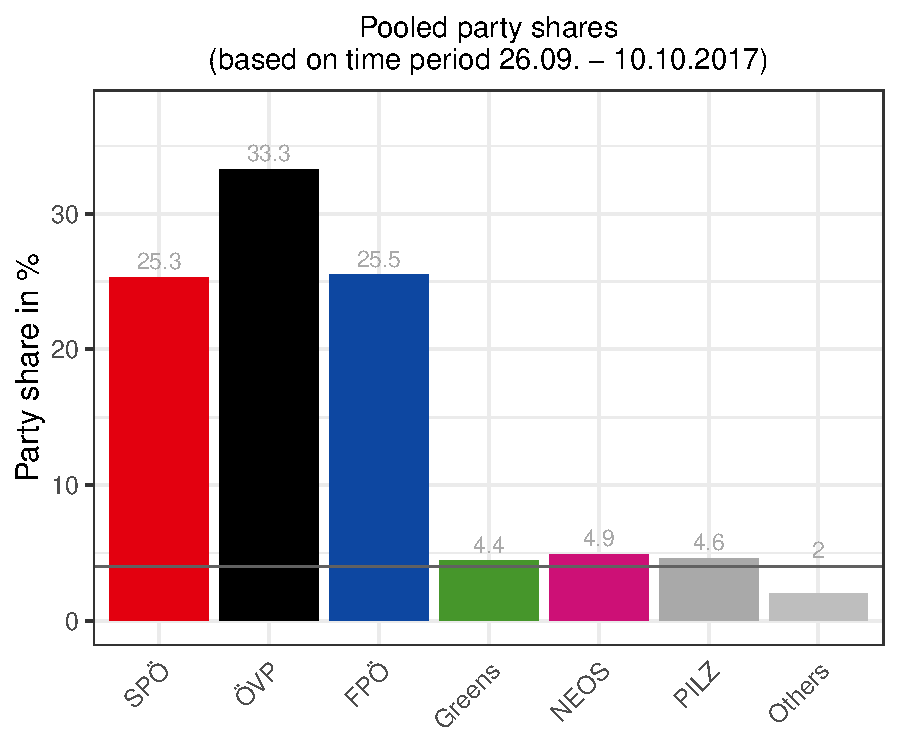
\includegraphics[width=0.6\textwidth]{figures/austria}
\end{center}

This situation resulted in only two-party coalitions having relevant (and very stable) probabilities to achieve joint majorities. A discussion of more complex three-party coalitions based on the development in Austria would not be fruitful as these generally had only very small POEs.
Taking into account all this information we now completely removed the Austria references from the paper.

  \item I would also like to see a table of the last estimates of some POEs with 90 or 95\% posterior intervals and the true outcomes in the application section.
  \\ \\
  \blue{Answer} We see your point regarding the missing evaluation of the POE approach based on real data.
However -- following what we outlined in the new subchapter 2.4 -- an inclusion of such a comparison of the last pre-election polls with the final election result would only be adequate to quantify the \emph{for-casting} error of our approach. If we were to include such a comparison, we see the danger that readers would confuse for-casting and now-casting to some extent. Hence, we decided not to include the comparison in the paper in order to clearly distinguish these two subjects.\\
Still, even though we did not include the evaluation in the paper, a comparison of the now-casts and the final election outcome can be found in the following table. The comparison is mainly based on the events discussed in the paper. Be aware that observed differences can be due to a misspecification of our model as well as shifts in the electorate shortly before election day.
\end{enumerate}

\begin{center}
\renewcommand{\arraystretch}{1.1} % Zeilenhöhe anpassen
\begin{tabular}{|cl|cc|cc|} \hline
\multicolumn{1}{|c}{\cellcolor{gray!25}} & \cellcolor{gray!25} & \multicolumn{2}{c|}{\cellcolor{gray!25}POE evaluation} & \multicolumn{2}{c|}{\cellcolor{gray!25}Share evaluation} \\
\cellcolor{gray!25}\multirow{-2}{*}{Election} & \cellcolor{gray!25}\multirow{-2}{*}{Event} & \cellcolor{gray!25}POE & \cellcolor{gray!25}Occurrence & \cellcolor{gray!25}$95\%$ CI$_{share}$ & \cellcolor{gray!25}Share \\ \hline
\multirow{6}{*}{2013} & Joined majority of Union-FDP & $28\%$ & - & $[42.1\%,46.4\%]$ & $41.5\%$ \\
& Joined majority of SPD-Left-Greens & $57\%$ & \ding{51} & $[42.8\%,47.2\%]$ & $42.7\%$ \\
& Greens third strongest party & $47\%$ & - & $[7.7\%,10.3\%]$ & $8.4\%$ \\
& Left third strongest party & $53\%$ & \ding{51} & $[7.7\%,10.4\%]$ & $8.6\%$ \\
& FDP passing into parliament & $89\%$ & - & $[4.7\%,6.8\%]$ & $4.8\%$ \\
& AfD passing into parliament & $12\%$ & - & $[3.5\%,5.4\%]$ & $4.7\%$ \\ \hline
\multirow{5}{*}{2017} & Joined majority of Union-FDP & $0.2\%$ & - & $[43.0\%,46.9\%]$ & $43.6\%$ \\
& SPD-Left-Greens & $<0.1\%$ & - & $[37.0\%,41.0\%]$ & $38.6\%$ \\
& AfD third strongest party & $93\%$ & \ding{51} & $[10.1\%, 12.7\%]$ & $12.6\%$ \\
& Left third strongest party & $5\%$ & - & $[8.6\%,11.1\%]$ & $9.2\%$ \\
& FDP third strongest party & $2\%$ & - & $[8.2\%,10.6\%]$ & $8.9\%$ \\

\hline
\end{tabular}
\captionof{table}{Comparison of now-casts and the final election outcome based on selected events. POEs (column \emph{POE}) are compared to the indicator if the event did occur (\emph{Occurrence}), $95\%$ credibility intervals for the (joint) party shares (\emph{$95\%$ CI$\_{share}$}) are compared to the final party shares in the election (\emph{Share}). The events relate to the 2013 and 2017 German federal elections that took place on 22.09.2013 and 24.09.2017, respectively. For the estimation a pooled sample was used (with time period 05.09.2013 to 19.09.2013 and 08.09.2017 to 22.09.2017, respectively) and 10\,000 simulations were performed.
}
\end{center}

As can be seen, most credibility intervals for the party shares include the final outcome. A difference between the now-cast and the final result can be observed in the 2013 joined party shares of Union-FDP and SPD-Left-Greens. Also, all POEs $>50\%$ ($<50\%$) apart from one are associated with an (no) occurrence of the corresponding event. Only in the 2017 case of the FDP passing into parliament there was a now-casted $89\%$ chance for the party to succeed, but in the end FDP ended up slightly below the necessary $5\%$ hurdle.


%----------- Second reviewer
\pagebreak
\begin{center}
\large Response to Reviewer \#2
\end{center}
\vspace{5ex}

The authors provide an interesting contribution to the estimation of probabilities of events (POE) in the context of now-casts of coalitions in parliaments. Their approach bases on the regularly published results of polling institutes. The methodology uses a Bayesian framework with the Multinomial distribution and a non-informative Dirichlet distribution as a prior. Also rounding to integer percentages is considered. The core of the procedure is a simulation of voting results of the basis of repeated draws from the posterior distribution of party shares. The procedure can be realized by an R-package. As a by-product the manuscript presents also some attractive ways to display the POEs. The use of these techniques is demonstrated by four examples from the last general election of the German Bundestag.
\\ \\
The proposed technique is well suited to improve the practice of now-casts. The manuscript is clearly written. The figures are illustrative.
\\ \\
There are only some minor details to be mentioned.

\section*{Comments}
\begin{enumerate}
  \item The authors mention possible deviations from the assumed Multinomial distribution.
  \begin{itemize}
    \item One example is a possible correlation of the count numbers from the different polling institutes. This is reflected by the authors by the so-called effective sample size when data from different polling institutes are pooled. One way to check such correlation might be to compare the now-casts with the realized voting results. Therefore it might be also fruitful to display the prediction error of the polling institutes.
    \item Another source of deviation from the Multinomial distribution might arise from the sampling procedures of surveys. Here the so-called design defect refers to the increase of the variance with respect to the binomial variance.
    \item Also the weighting procedures are prone to increase the variance of the population estimates.
  \end{itemize}
  So there are good reasons to suspect the Multinomial distribution even in the case of case numbers from a single polling institute. Admittedly, the polling
institutes do not publish such details. However, one should be cautious with the Multinomial distribution assumption. One way to demonstrate a possible under-estimation of the variance is to display the realized voting results together with its posterior distribution.
  \\ \\
  \blue{Answer} As both reviewers made a similar point we allow ourselves to simply repeat the answer to the comment of reviewer \#1 as first part of the answer: \\
Thank you for the detailed feedback! We have to admit that this is something we did not discuss
thoroughly enough. We now added the new subchapter 2.4 for this discussion of potential biases -- both resulting from house biases or an industry bias and from specific survey designs (comprising the sampling design and the post-sampling weighting scheme). As in both cases the bias quantification for our \emph{now-casting} approach is hardly doable with the given information, we decided to not adjust our approach further. \\
As stated in the new subchapter, when working with data from an individual polling agency, an adjustment does not seem crucial as the sample uncertainty induced by our Multionmial approach matches the uncertainty communicated by the individual German polling agencies that we use.\\

Additionally, you propose the evaluation of the approach based on final election outcomes. Again, we refer to the detailed answer we gave to the third comment of reviewer \#1 as both of you made comparable comments. There, we outline why we did not include such a quantification of the for-casting error in the paper and shortly evaluate the method for the 2013 and the 2017 German federal elections.

  \item page 3, paragraphs 2 and 3: Austria is  mentioned two times but no example from Austria is displayed. From my point of view the German examples are sufficient. Hence, one could skip the references to Austria.
  \\ \\
  \blue{Answer} Yes, mentioning Austria as an application example without showing results was redundant. We removed it from the paper.
  
  \item page 6, line 10: Something is wrong with the first citation in the bracket.
  \\ \\
  \blue{Answer} Thank you for the hint. We clarified the citation.
\end{enumerate}

\end{document}
